\documentclass[12pt,a4paper,utf8x]{report}
\usepackage [frenchb]{babel}
\usepackage[utf8]{inputenc}  
\usepackage[T1]{fontenc} 
% Pour pouvoir utiliser 
\usepackage{ucs}

\usepackage{textcomp}
\usepackage{graphicx}
\usepackage{keystroke}
\usepackage{amssymb}
\usepackage{amsmath}
\usepackage{listings}
%\usepackage{pifont}

\usepackage{url} % Pour avoir de belles url
\usepackage {geometry}

% Pour mettre du code source
\usepackage {listings}
% Pour pouvoir passer en paysage
\usepackage{lscape}

% Pour pouvoir faire plusieurs colonnes
\usepackage {multicol}
% POur crééer un index
\usepackage{makeidx}
\usepackage{graphicx}
\makeindex

% Pour l'interligne de 1.5
\usepackage {setspace}
% Pour les marges de la page
\geometry{a4paper, top=2.5cm, bottom=3.5cm, left=1.5cm, right=1.5cm, marginparwidth=1.2cm}

\parskip=5pt %% distance entre § (paragraphe)
\sloppy %% respecter toujours la marge de droite 

% Pour les pénalités :
\interfootnotelinepenalty=150 %note de bas de page
\widowpenalty=150 %% veuves et orphelines
\clubpenalty=150 

%Pour la longueur de l'indentation des paragraphes
\setlength{\parindent}{15mm}



%%%% debut macro pour enlever le nom chapitre %%%%
\makeatletter
\def\@makechapterhead#1{%
  \vspace*{50\p@}%
  {\parindent \z@ \raggedright \normalfont
    \interlinepenalty\@M
    \ifnum \c@secnumdepth >\m@ne
        \Huge\bfseries \thechapter\quad
    \fi
    \Huge \bfseries #1\par\nobreak
    \vskip 40\p@
  }}

\def\@makeschapterhead#1{%
  \vspace*{50\p@}%
  {\parindent \z@ \raggedright
    \normalfont
    \interlinepenalty\@M
    \Huge \bfseries  #1\par\nobreak
    \vskip 40\p@
  }}
\makeatother
%%%% fin macro %%%%

%Couverture 


\title
{
	\normalsize{ M1 ALMA\\ 
	Université de Nantes\\
	2010-2011}\\
	\vspace{15mm}
	\Huge{Projet de TP n°2\\Structures complexes et algorithmes}
}



\author{MARGUERITE Alain\\ RINCE Romain
	\vspace{45mm}
}

\date
{	
	\normalsize{Université de Nantes \\ 2 rue de la Houssinière, BP92208, F-44322 Nantes cedex 03, FRANCE
	\\ 
	\vspace{5mm}	
	Encadrant : Christophe JERMANN \\
	}
}

\begin{document}

\maketitle


\clearpage

\tableofcontents
\clearpage

% Pour avoir un interligne de 1,5
\begin{onehalfspace}
\chapter{Introduction}

\renewcommand{\labelitemi}{$\bullet$}
\section{Problème à résoudre}
L'objectif de ce projet est de réaliser un Global Positioning System «amélioré». Sans entrer dans les détails, un GPS est réalisé à partir d'une modelisation sous forme de graphe orienté d'une carte où les posistions sont des noeuds et les routes sont des arcs. L'application d'algorithmes de plus courts chemins sur ces graphes permettent alors de répondre au problème concrét du calcul d'iténéraires. Cependant il est rare, dans la vie réelle, que ce type de problème admette une unique contrainte. Ici nous allons travailler sur des graphes plus complexes (voir figure ci-après) par leurs nombres de paramètres
\begin{figure}[!h] 
\begin{center}
  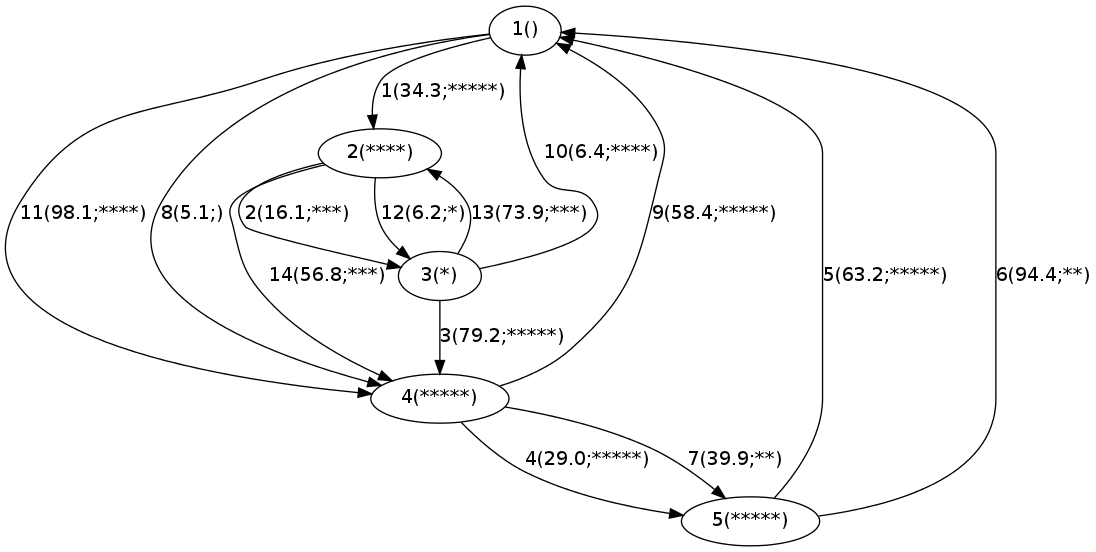
\includegraphics[scale=0.40]{g.png}
\end{center}
\end{figure} 

L'idée de réaliser un GPS prenant aussi en compte l'aspect touristique d'un lieu ou d'une route donne les opportunités suivantes : 
\begin{itemize}
\item
Une étude approfondie des algorithmes sur les graphes étudiés en cours pour choisir le plus adapté en fonction du problème et de la structure de donnée concrète.
\clearpage
\item
Des manipulations plus complexes de ces algorithmes puisqu'ils prennent plusieurs (et non un seul) paramètres en compte.
\item
Ces différents choix de combinaisons d'implémentations et d'algorithmes entraînes des calculs variés.
\end{itemize}

Tous ces aspects sont au coeur même du module Structures complexes et algorithmique. La première partie du projet se contentait d'étudier et d'implémenter des structures et des algorithmes complexes. Au terme de l'ultime partie, nous réalisons à partir de ces outils  théoriques une application concrète.

\clearpage

\section{Application réalisée}

\subsection{Structure du programme}
Dans la continuité de la première partie du projet, nous avons conçu de nouvelles classes en nous appuyant sur celles de notre graphe orienté. Voici la liste des différents fichiers du package GPS : 

\begin{itemize}
\item
Ville.java : Composée d'un nom et d'une entier qualilté dénombrant le nombre d'étoiles
\item
Route.java : Héritant de la classe Arc.java, posède un plus une longueur  et d'une qualité tout comme Ville.java
\item
GPS.java : Comporte les différentes méthodes demandées dans le sujet. Le constructeur prend en compte les données fournies par le parseur ainsi que celle saisie sur l'entrée standards par l'utilisateur
\item
Parser.java : Parse le fichier fourni en paramètre et retourne à la classe appelante le graphe créé ainsi que la distance max entre deux villes sur le graphe, la meilleure qualité, et un annuaire inversé qui donne l'id d'un nœud ou d'un arc dans le graphe à partir de son nom.
\end{itemize}


\subsection{Déroulement de l'application}
Le programme se lance sans paramètres. Il demande à l'utilisateur d'entrer successivement : 
\begin{itemize}
\item
Le nom du fichier d'entrée (devant être présent dans le dossier courant).
\item
Le choix d'implémentation (l la liste d'adjacence et m pour la matrice d'adjacence).
\item
Le nom de la ville de départ.
\item
Le nom de la ville d'arrivée.
\item 
La valeur (K ou A) du paramètre en fonction de la méthode choisie.
\end{itemize}
L'itinéraire calculé sera alors affiché selon les consignes du sujet. Le programme se termine par la suite. Il faut relancer le programme un autre calcul?
 


\chapter{PARTIE2}
\section{Algorithme de plus court chemin}
Les deux methodes demandées pour le calul d'itinéaire (par agrégation et à détour borné), il est necessaire  d'employer un algoritme de plus court chemin.
Notre choix de d'algorithme s'est orienté vers celui Bellman Ford. Son avantage par rapport à celui de Dijkstra est qu'il est capable de détecter un circuit absorbant. Il peut de la sorte informer l'utilisateur l'echec de a recherche d'un itinéraire compromis selon ces paramètres. 

IMPLEMENTATION DE DIJKSTRA QUAND MEME ??


\section{Methode Agrégation}
L'objectif de cette methode est d'obtenir un plus court chemin avec une pondération particulière pour routes calculée au préalable.
Il suffit donc d'appliquer un algorithme standard de parcours de graph en fournissant toutes les pondérations de chaques routes et villes que l'on aura calculé au préalable. N Nous avons procédé de cette manière. Ainsi la fonction $get_agregat(Route route, double A)$ permet de donner l'agrégat d'une route. Elle est utilisée par  $public ArrayList<Double> agregation(double A)$ qui retourne un tableau de ces pondération indicé par l'id des routes. Ce tableau est ensuite fourni en paramètre à l'Algorithme de Bellman Ford. Celui ci pourra alors procéder au relâchement des arcs en fonctions de ces pondérations. 

 
Méthode d’agrégation
La méthode d’agrégation consiste à considérer une fonction de pondération w des arcs du graphe
qui est calculée à partir des décorations des nœuds et arcs de celui-ci. Une fois cette fonction définie, le
problème devient un simple problème de plus court chemin et peut alors être résolu par les algorithmes
vus en cours 1 . La fonction w peut être définie comme une fonction d’agrégation des deux critères distance
(d) et intérêt (i) :
wA (u → v) = A ∗ d(u → v)/dmax − (1 − A) ∗ (i(u → v) + i(v))/(2 ∗ imax )
(1)
où dmax est la plus grande distance affectée à une route, imax est le plus grand intérêt porté à un lieu ou
à une route, et A est un paramètre réel compris en 0 et 1 qui représente l’importance respective donnée
à la distance par rapport à l’intérêt touristique : lorsque A = 0 le chemin calculé dépend uniquement
de l’intérêt, alors que lorsque A = 1 il ne dépend que de la distance. L’intérêt d’une route est toujours
additionnée à celui du lieu auquel elle conduit : les lieux traversés sont visités et augmentent donc l’attrait
touristique de l’itinéraire. Les termes dmax et imax interviennent ici afin de normaliser les deux critères
relativement l’un à l’autre : après normalisation, la distance et l’intérêt de tout arc est un réel entre 0 et 1.
Ces valeurs normalisées et pondérées par leurs importances respectives sont alors agrégées par différence,
du fait de leur nature contradictoire : le long d’un chemin, l’intérêt augmente nécessairement lorsque la
distance augmente, et diminue nécessairement lorsqu’elle diminue ; or il faut minimiser la distance tout
en maximisant l’intérêt. Notez que selon la valeur de A, la pondération wA de certains arcs pourrait être
négative, et le graphe pourrait même contenir un circuit absorbant ! Dans ce cas, cette méthode échoue
et ne peut calculer un itinéraire compromis.


\clearpage

\chapter{Analyse théorique}
\section{BLA}
BLABLABLABLABLABLABLABLABLA

\section{Conclusion}%% methode la plus efficace
BLABLABLABLA


\clearpage



\chapter{Analyse experimentale}
\section{Introduction}
Tous nos tests sont effectués en respectant les démarches suivantes : 
\begin{itemize}
\item
Les relevés temporels sont ceux de l'utilisation CPU. Dans un soucis de minimiser les facteurs faussant les relevés (impacts d'autres processus actifs), nous avons essayé d'avoir un minimun de processus actifs pendant les relevés.
\item
Chaques tests a été effectué 3 fois. Le resultat final étant la moyenne de ces trois tests.
\item
Les tests ont pour objectif de confronter nos raisonement lors de l'analyse théorique (cf : )
\item
ROMAIN ROAMIN




\end{itemize}
\section{BLA}

%– une analyse expérimentale de la complexité temporelle des algorithmes présentés. Cette étude com-
%parera en particulier l’impact du choix de telle ou telle structure sur les méthodes implémentées.
%Elle sera réalisée sur des cartes routières variant de quelques dizaines à plusieurs milliers de nœuds
%et établira l’influence des paramètres tels que la densité du graphe, la diversité des décorations,
%etc. Cette analyse sera mise en regard de l’étude théorique et les éventuels écarts observés seront
%expliqués.
BLABLABLABLA



\section{Conclusion}%% methode la plus efficace
BLABLABLABLA




% Pour finir l'interligne de 1,5
\end{onehalfspace}

\printindex

\appendix


\end{document}
